\subsection{Comparison with external morphology catalogues}
\label{sec:results_external}

We compare the ensemble assignments with the mapped labels of \citet{Clews2025}, \citet{Horton2025}, and \citet{Chilufya2025}, using the correspondences in Sec.~\ref{sec:method_external_mapping}. The mapped samples in Table~\ref{tab:external_individual_samples} include \(645\), \(718\), and \(198\) members of the internally curated subsample, respectively. These comparisons assess agreement with independently compiled label schemes, not an established physical ground truth. FRII includes both Edge-bright FRII and Large FRII throughout the comparison.

The main findings remain after excluding all curated sources (Table~\ref{tab:excluded_curated}). The figures retain the full mapped samples; Appendix~\ref{app:evaluation} gives additional checks. The exclusion removes overlap with supervised training, although these sources still participated in pre-training.
This check uses the curated-excluded selections in the final column of Table~\ref{tab:external_individual_samples}.

\begin{table}[H]
\centering
\small
\setstretch{1}
\setlength{\tabcolsep}{8pt}
\renewcommand{\arraystretch}{1.6}
\begin{tabular}{@{}lrrr@{}}
\toprule
Catalogue & Sources & FRI \(F_1\) & FRII \(F_1\) \\
\midrule
Clews & 7757 & \(0.389_{-0.021}^{+0.020}\) & \(0.735_{-0.013}^{+0.013}\) \\
Horton & 8352 & \(0.281_{-0.022}^{+0.020}\) & \(0.743_{-0.010}^{+0.010}\) \\
Chilufya & 2590 & \(0.445_{-0.036}^{+0.036}\) & \(0.455_{-0.033}^{+0.032}\) \\
\bottomrule
\end{tabular}

\caption[External correspondence excluding curated sources]{External correspondence after excluding all curated sources. Signed uncertainties give the distances to the \(95\,\%\) interval bounds.}
\label{tab:excluded_curated}
\end{table}

Figure~\ref{fig:ext_confusion_fri} shows the class correspondence for all three catalogues. We then examine FRI and FRII separately.

\begin{figure}[H]
\centering
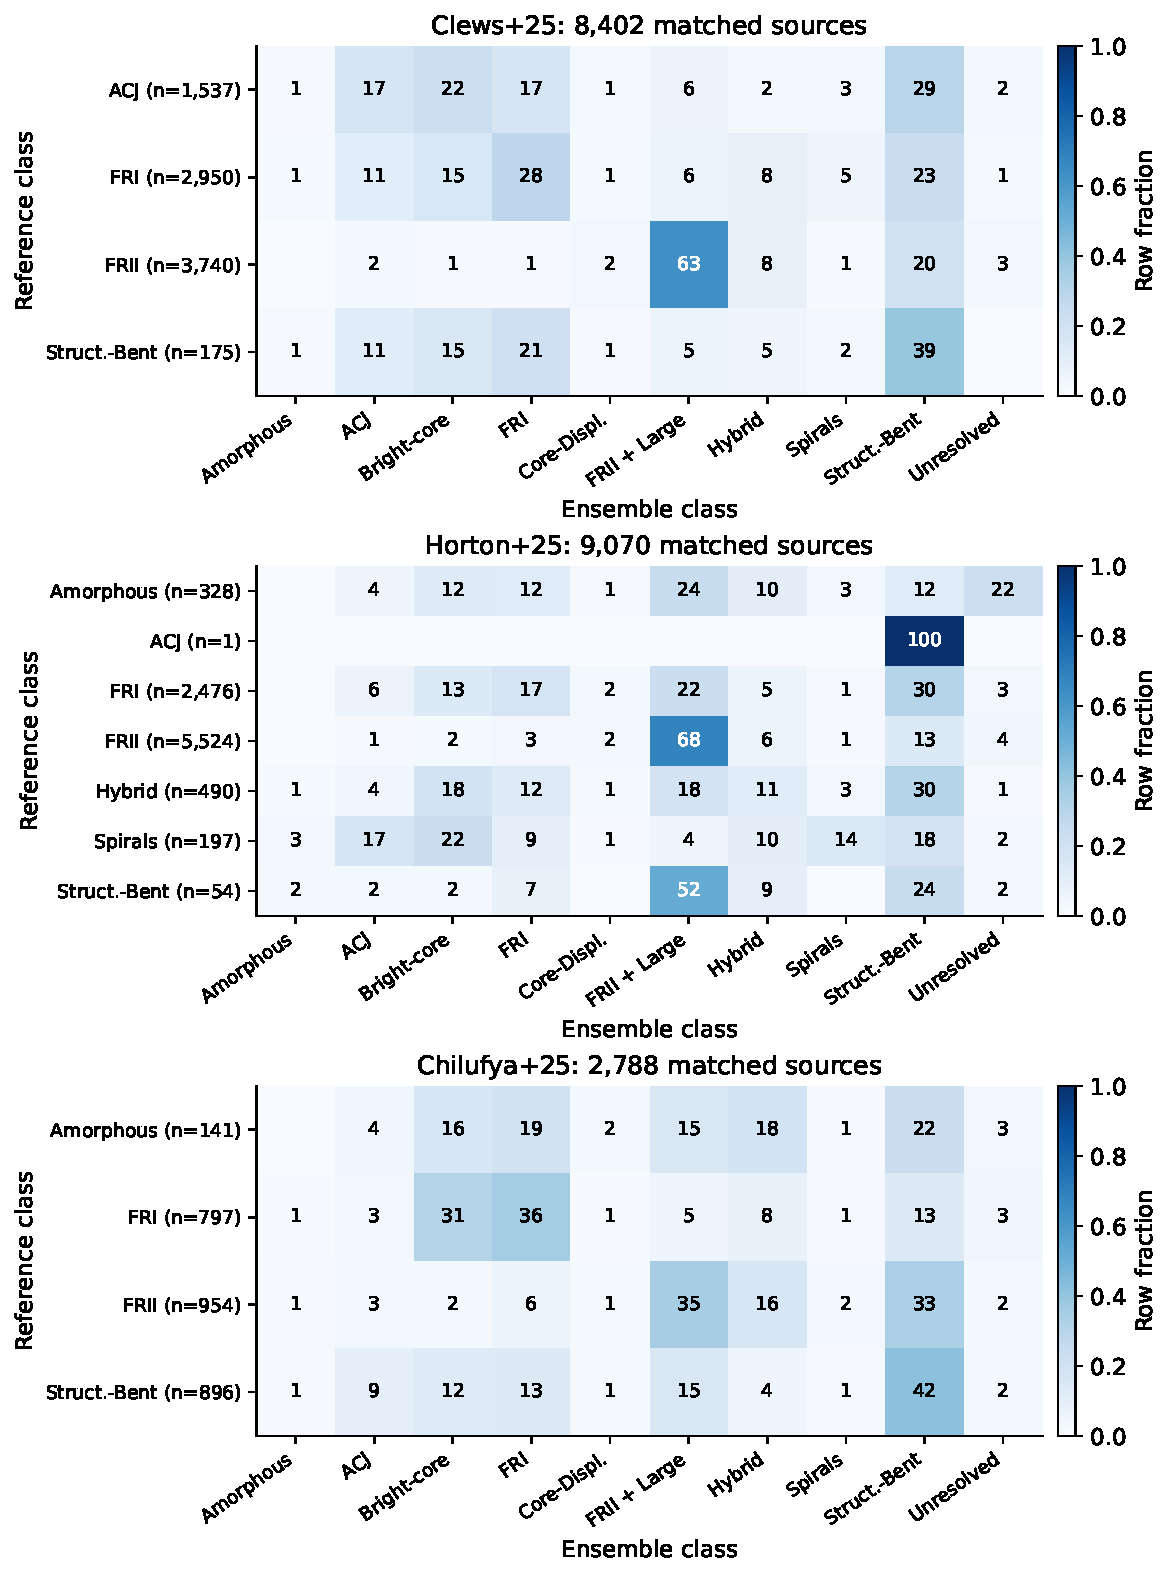
\includegraphics[width=\linewidth,height=0.87\textheight,keepaspectratio]{img/ext_confusion_FRII-relaxed.pdf}
\caption[Class correspondence with external catalogues]{Row-normalised class correspondence for Clews, Horton, and Chilufya. Rows are reference classes with source counts in parentheses; columns are ensemble predictions. Edge-bright FRII and Large FRII predictions are combined. Cells above \(0.5\,\%\) are annotated with percentages; reference classes absent from a catalogue are omitted.}
\label{fig:ext_confusion_fri}
\label{fig:ext_confusion_frii_r}
\end{figure}

\subsubsection{FRI correspondence}
\label{sec:ext_fri}

The model recovers FRI morphology poorly across all three catalogues (Table~\ref{tab:ext_fri}).

\begin{table}[H]
\centering
\small
\setlength{\tabcolsep}{4pt}
\setstretch{1}
\renewcommand{\arraystretch}{1.6}
\begin{tabular}{@{}lrrrrr@{}}
\toprule
Catalogue & Reference sources & TP & FP & FN & \(F_1\) \\
\midrule
Clews & 2950 & 818 & 334 & 2132 & \(0.399_{-0.019}^{+0.019}\) \\
Horton & 2476 & 431 & 278 & 2045 & \(0.271_{-0.020}^{+0.020}\) \\
Chilufya & 797 & 285 & 198 & 512 & \(0.445_{-0.035}^{+0.033}\) \\
\bottomrule
\end{tabular}

\caption[FRI agreement with external catalogues]{FRI agreement with the mapped reference labels; uncertainties indicate \(95\,\%\) intervals.}
\label{tab:ext_fri}
\end{table}

Frequent Bright-core assignments suggest that central brightness dominates over extended jets and lobes, while Structured-Bent assignments reveal sensitivity to bending (Figure~\ref{fig:ext_fn_fri}). These patterns also reflect catalogue-dependent class boundaries, particularly Horton's inclusion of curved sources within FRI \citep{Horton2025}.

\begin{figure}[H]
\centering
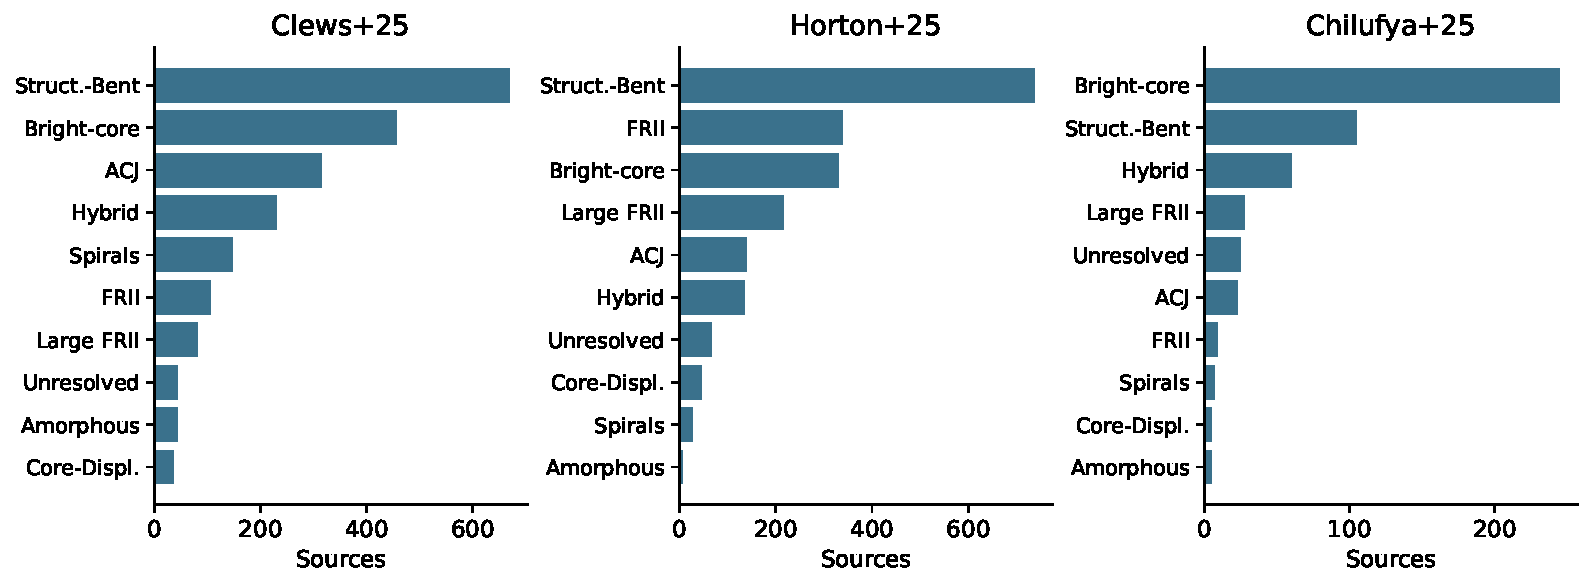
\includegraphics[width=\linewidth]{img/ext_fn_breakdown_FRI.pdf}
\caption[Predicted classes of missed reference FRI sources]{Ensemble assignments of reference FRI sources not predicted as FRI.}
\label{fig:ext_fn_fri}
\end{figure}

The ensemble also assigns alternative morphologies to reference FRI sources with high confidence (Figure~\ref{fig:ext_conf_fri}).

\begin{figure}[H]
\centering
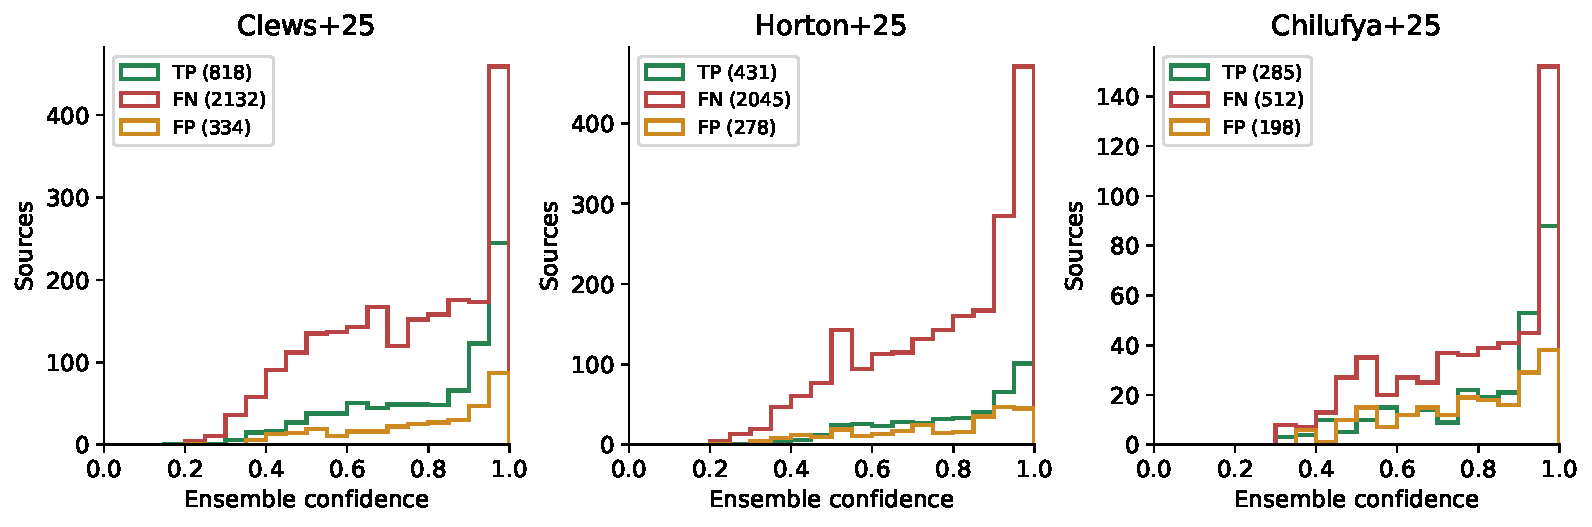
\includegraphics[width=\linewidth]{img/ext_confidence_FRI.pdf}
\caption[Ensemble confidence in the FRI comparisons]{Ensemble confidence for FRI true positives, false negatives, and false positives relative to each reference catalogue.}
\label{fig:ext_conf_fri}
\end{figure}

\subsubsection{FRII correspondence}
\label{sec:ext_frii}

FRII correspondence is strongest against Clews and Horton and weaker against Chilufya (Table~\ref{tab:ext_frii}).

\begin{table}[H]
\centering
\small
\setlength{\tabcolsep}{4pt}
\setstretch{1}
\renewcommand{\arraystretch}{1.6}
\begin{tabular}{@{}lrrrrr@{}}
\toprule
Catalogue & Reference sources & TP & FP & FN & \(F_1\) \\
\midrule
Clews & 3740 & 2359 & 287 & 1381 & \(0.739_{-0.012}^{+0.012}\) \\
Horton & 5524 & 3744 & 759 & 1780 & \(0.747_{-0.010}^{+0.010}\) \\
Chilufya & 954 & 333 & 192 & 621 & \(0.450_{-0.032}^{+0.032}\) \\
\bottomrule
\end{tabular}

\caption[FRII agreement with external catalogues]{FRII agreement with the mapped reference labels; uncertainties indicate \(95\,\%\) intervals.}
\label{tab:ext_frii}
\end{table}

Against Chilufya, FRI and FRII performance is similar, including after curated-source exclusion.

The remaining disagreements concentrate in Structured-Bent and Hybrid across all three catalogues (Figure~\ref{fig:ext_fn_frii}). This pattern suggests that curvature and mixed brightening patterns complicate the model's recognition of edge-brightened FRII structure.

\begin{figure}[H]
\centering
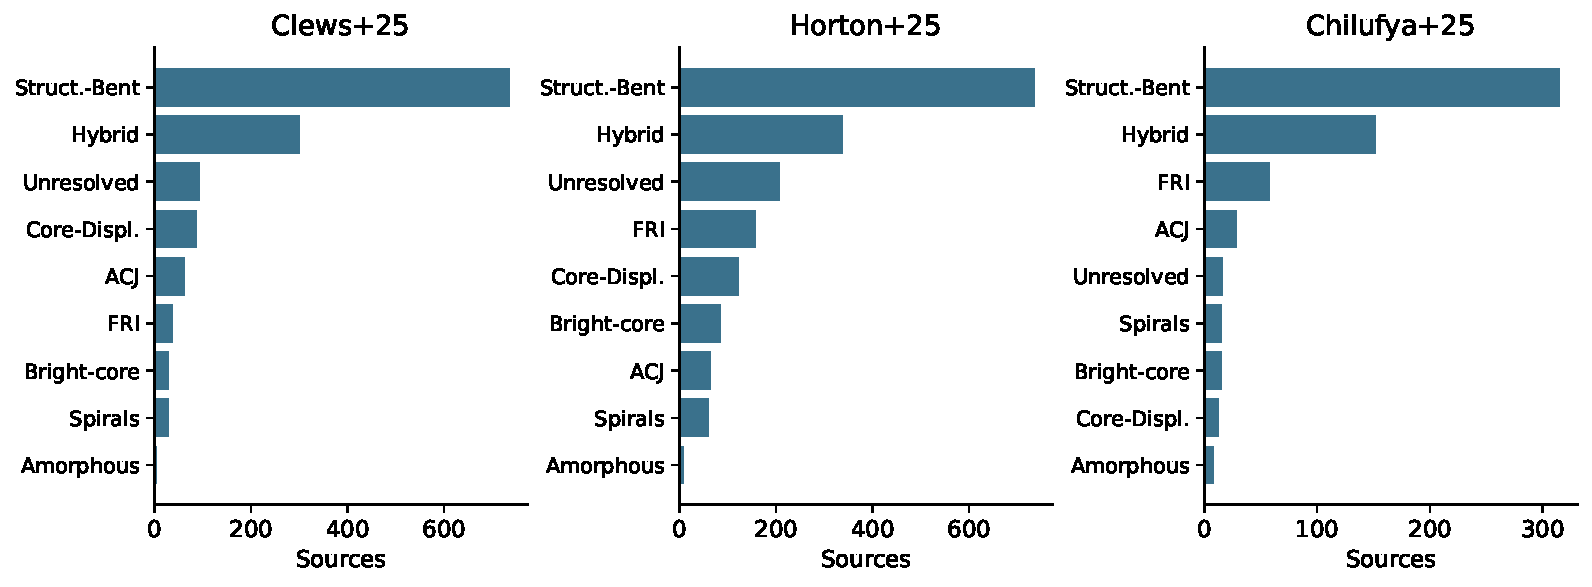
\includegraphics[width=\linewidth]{img/ext_fn_breakdown_FRII-relaxed.pdf}
\caption[Predicted classes of missed reference FRII sources]{Ensemble assignments of reference FRII sources predicted as neither Edge-bright FRII nor Large FRII.}
\label{fig:ext_fn_frii}
\end{figure}

Reference FRII sources assigned to either internal FRII class have higher median confidence than those assigned to other classes (Figure~\ref{fig:ext_conf_frii}).

\begin{figure}[H]
\centering
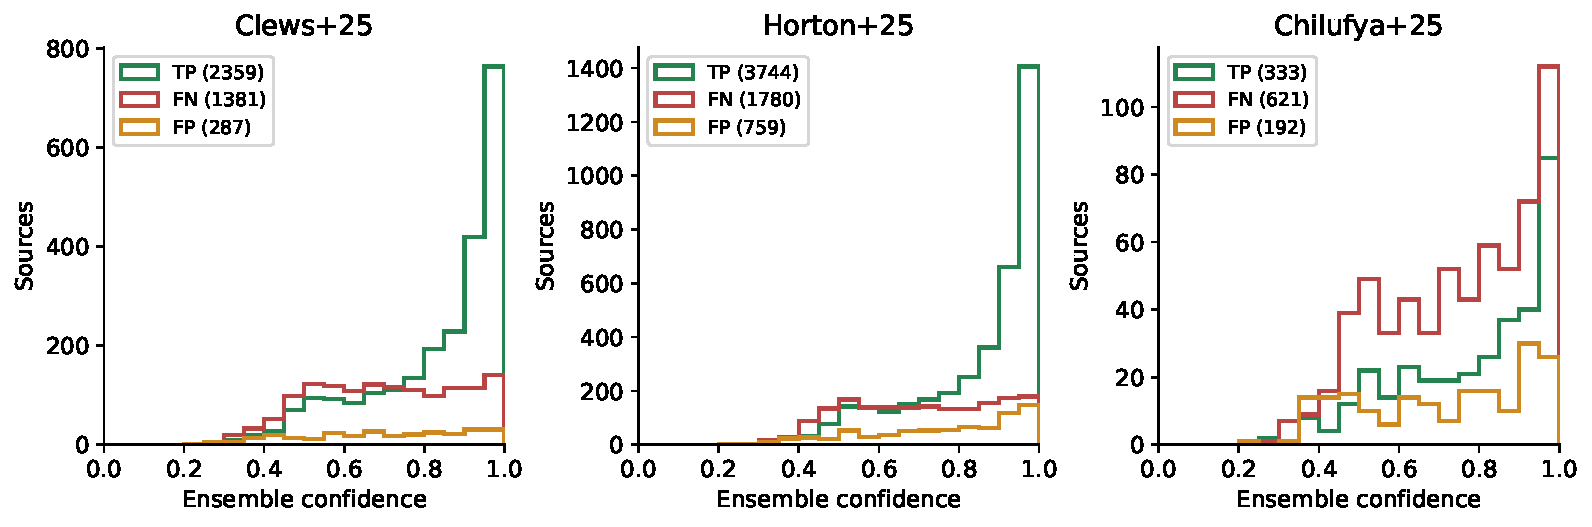
\includegraphics[width=\linewidth]{img/ext_confidence_FRII-relaxed.pdf}
\caption[Ensemble confidence in the FRII comparisons]{Ensemble confidence for FRII true positives, false negatives, and false positives.}
\label{fig:ext_conf_frii}
\end{figure}

\subsubsection{Three-catalogue consensus}
\label{sec:ext_consensus}

Of the sources in the common-source sample defined in Table~\ref{tab:external_combined_samples}, \(311\) have usable mapped labels in all three references. Of these, \(149\) receive the same mapped label, forming the consensus subset independently of the ensemble predictions; ten belong to the curated subsample. The ensemble agrees with the common reference label for fewer than half of these sources (Table~\ref{tab:ext_consensus}).

\begin{table}[H]
\centering
\small
\setlength{\tabcolsep}{5pt}
\setstretch{1}
\renewcommand{\arraystretch}{1.6}
\begin{tabular}{@{}lrrrrr@{}}
\toprule
Reference class & Sources & TP & FP & FN & \(F_1\) \\
\midrule
FRI & 62 & 25 & 0 & 37 & \(0.575_{-0.136}^{+0.117}\) \\
FRII & 87 & 43 & 4 & 44 & \(0.642_{-0.104}^{+0.090}\) \\
\bottomrule
\end{tabular}

\caption[Agreement with three-catalogue consensus labels]{Agreement with labels shared by all three catalogues; uncertainties indicate \(95\,\%\) intervals.}
\label{tab:ext_consensus}
\end{table}

Agreement remains below half after excluding the curated sources.
Reference FRI sources receive Bright-core assignments almost as often as FRI assignments, while reference FRII disagreements mainly involve Structured-Bent and Hybrid (Figure~\ref{fig:ext_consensus}).
\begin{figure}[H]
\centering
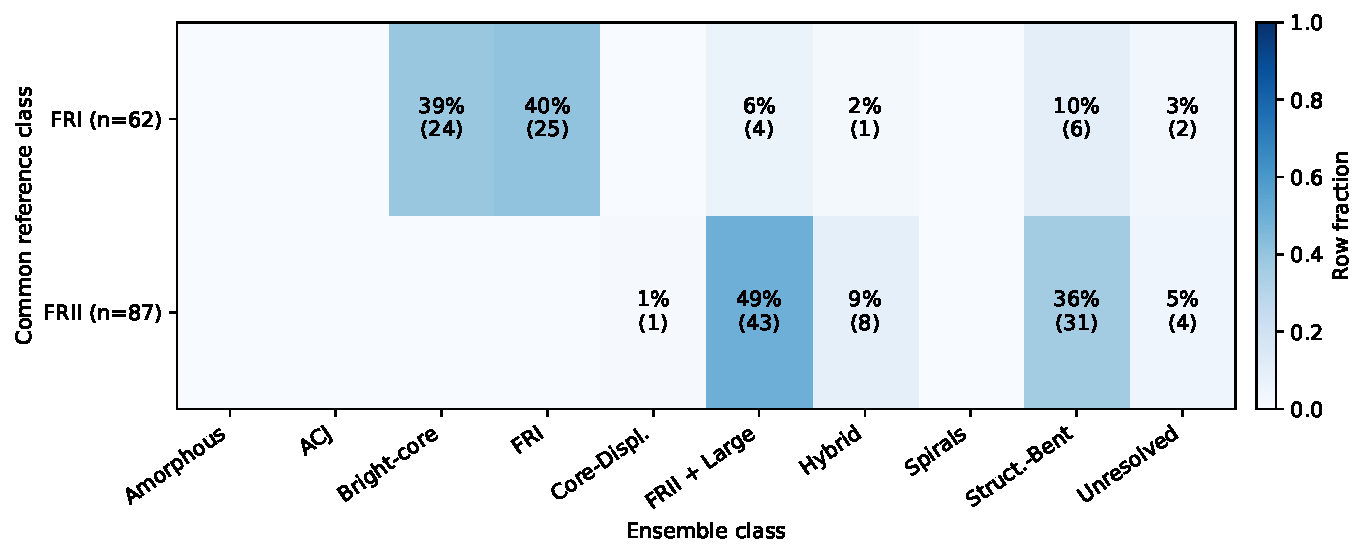
\includegraphics[width=0.8\linewidth]{img/ext_confusion_consensus.pdf}
\caption[Predicted classes of three-catalogue consensus sources]{Ensemble assignments for the \(149\) three-catalogue consensus sources. Cells give row percentages and source counts.}
\label{fig:ext_consensus}
\end{figure}

\subsubsection{\texorpdfstring{\(S_\mathrm{RG}\)}{S\_RG} distribution across mapped-reference sources}
\label{sec:ext_group_retention}
\label{sec:ext_gallery}
\label{sec:ext_summary}

Table~\ref{tab:ext_group_retention} includes all sources with a usable reference label in either \(G\) or \(N\). For each catalogue, we separate fine-class agreements from disagreements and report the ensemble's \(G/N\) assignments within each subset.

\begin{table}[h]
\centering
\small
\setlength{\tabcolsep}{4pt}
\begin{tabular}{@{}llrrrr@{}}
\toprule
Catalogue & Subset & Sources & \shortstack[r]{Share\\(\%)} & \shortstack[r]{Assigned to \(G\)\\\(n\) (row \%)} & \shortstack[r]{Assigned to \(N\)\\\(n\) (row \%)} \\
\midrule
Clews & All mapped & 8\,402 & 100.0 & 7\,943 (94.5) & 459 (5.5) \\
 & Agreements & 3\,501 & 41.7 & 3\,501 (100.0) & 0 (0.0) \\
 & Disagreements & 4\,901 & 58.3 & 4\,442 (90.6) & 459 (9.4) \\
\midrule
Horton & All mapped & 9\,070 & 100.0 & 8\,551 (94.3) & 519 (5.7) \\
 & Agreements & 4\,271 & 47.1 & 4\,244 (99.4) & 27 (0.6) \\
 & Disagreements & 4\,799 & 52.9 & 4\,307 (89.7) & 492 (10.3) \\
\midrule
Chilufya & All mapped & 2\,788 & 100.0 & 2\,670 (95.8) & 118 (4.2) \\
 & Agreements & 991 & 35.5 & 991 (100.0) & 0 (0.0) \\
 & Disagreements & 1\,797 & 64.5 & 1\,679 (93.4) & 118 (6.6) \\
\bottomrule
\end{tabular}
\caption[Group assignments for fine-class agreements and disagreements]{Fine-class correspondence for all mapped reference sources.}
\label{tab:ext_group_retention}
\end{table}

Figure~\ref{fig:ext_srg_distributions} shows the score components for the \(16\,177\) study sources with at least one mapped reference label (Table~\ref{tab:external_combined_samples}).
Each source is counted once, irrespective of catalogue overlap or agreement with the ensemble. 
For sources assigned to \(N\), the \(P_\mathrm{RG}\) distribution is concentrated towards low values, indicating weak support for radio-galaxy-like morphologies.
Their scores remain below \(S_\mathrm{RG}=0.25\), even where ensemble reliability is high.

\begin{figure}[H]
\centering
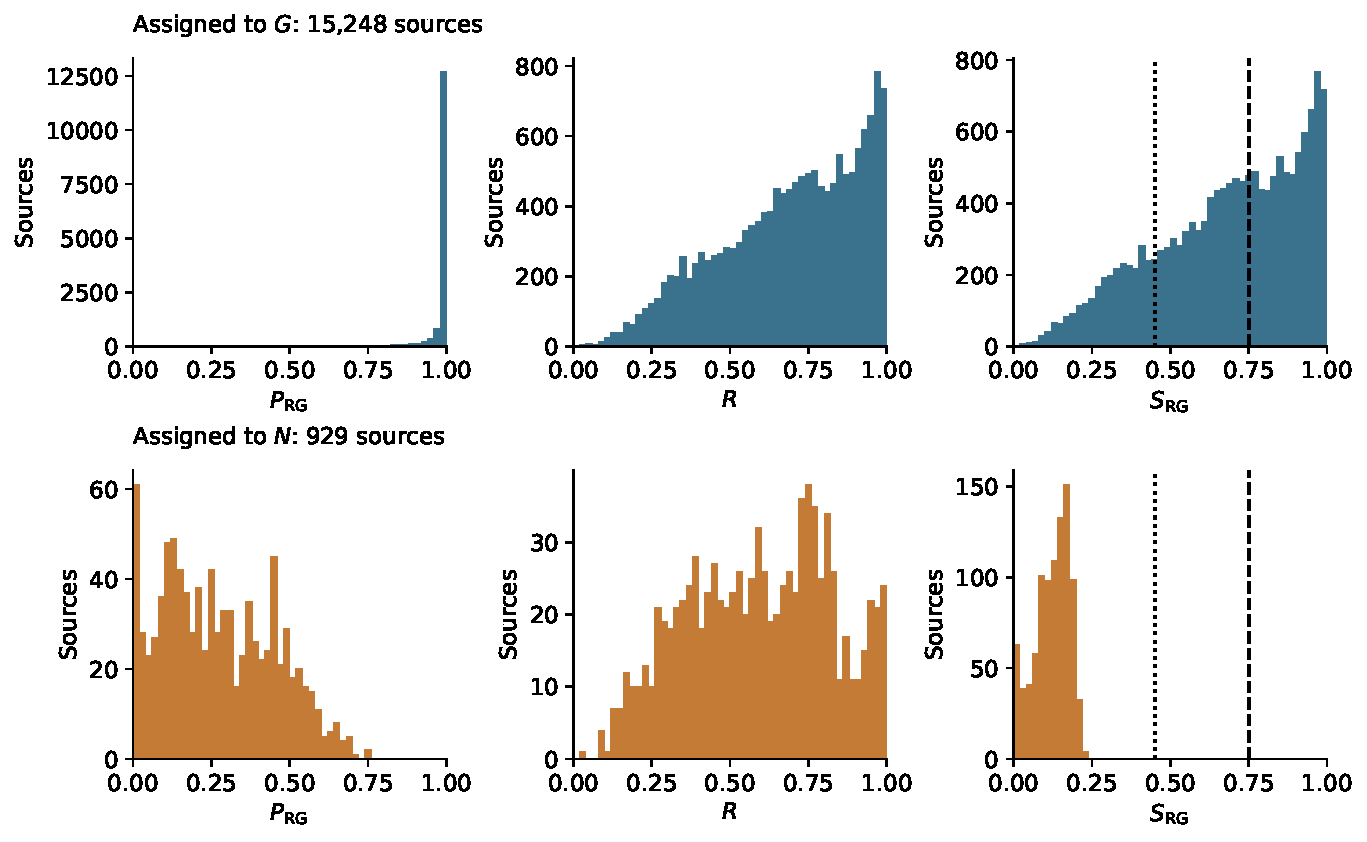
\includegraphics[width=\linewidth]{img/external_srg_distributions.pdf}
\caption[Score distributions for mapped-reference sources]{Score components for sources with mapped reference labels, separated by ensemble-assigned \(G\) (top) and \(N\) (bottom). Dashed and dotted lines mark \(S_\mathrm{RG}=0.75\) and \(0.45\).}
\label{fig:ext_srg_distributions}
\end{figure}

For the visual examples in Figure~\ref{fig:agree_gallery}, we select sources with at least one mapped reference label and agreement between every available mapped label and the ensemble assignment. We show five examples for each of six internal classes (ACJ, FRI, FRII, Hybrid, Spirals, and Structured-Bent).
We prioritise sources covered by more reference catalogues. These examples illustrate agreement without assuming its prevalence. In Appendix~\ref{app:external_disagreements} we present the complementary inspection sample (disagreement examples for each of the eleven internal classes).

\begin{figure}[H]
\centering
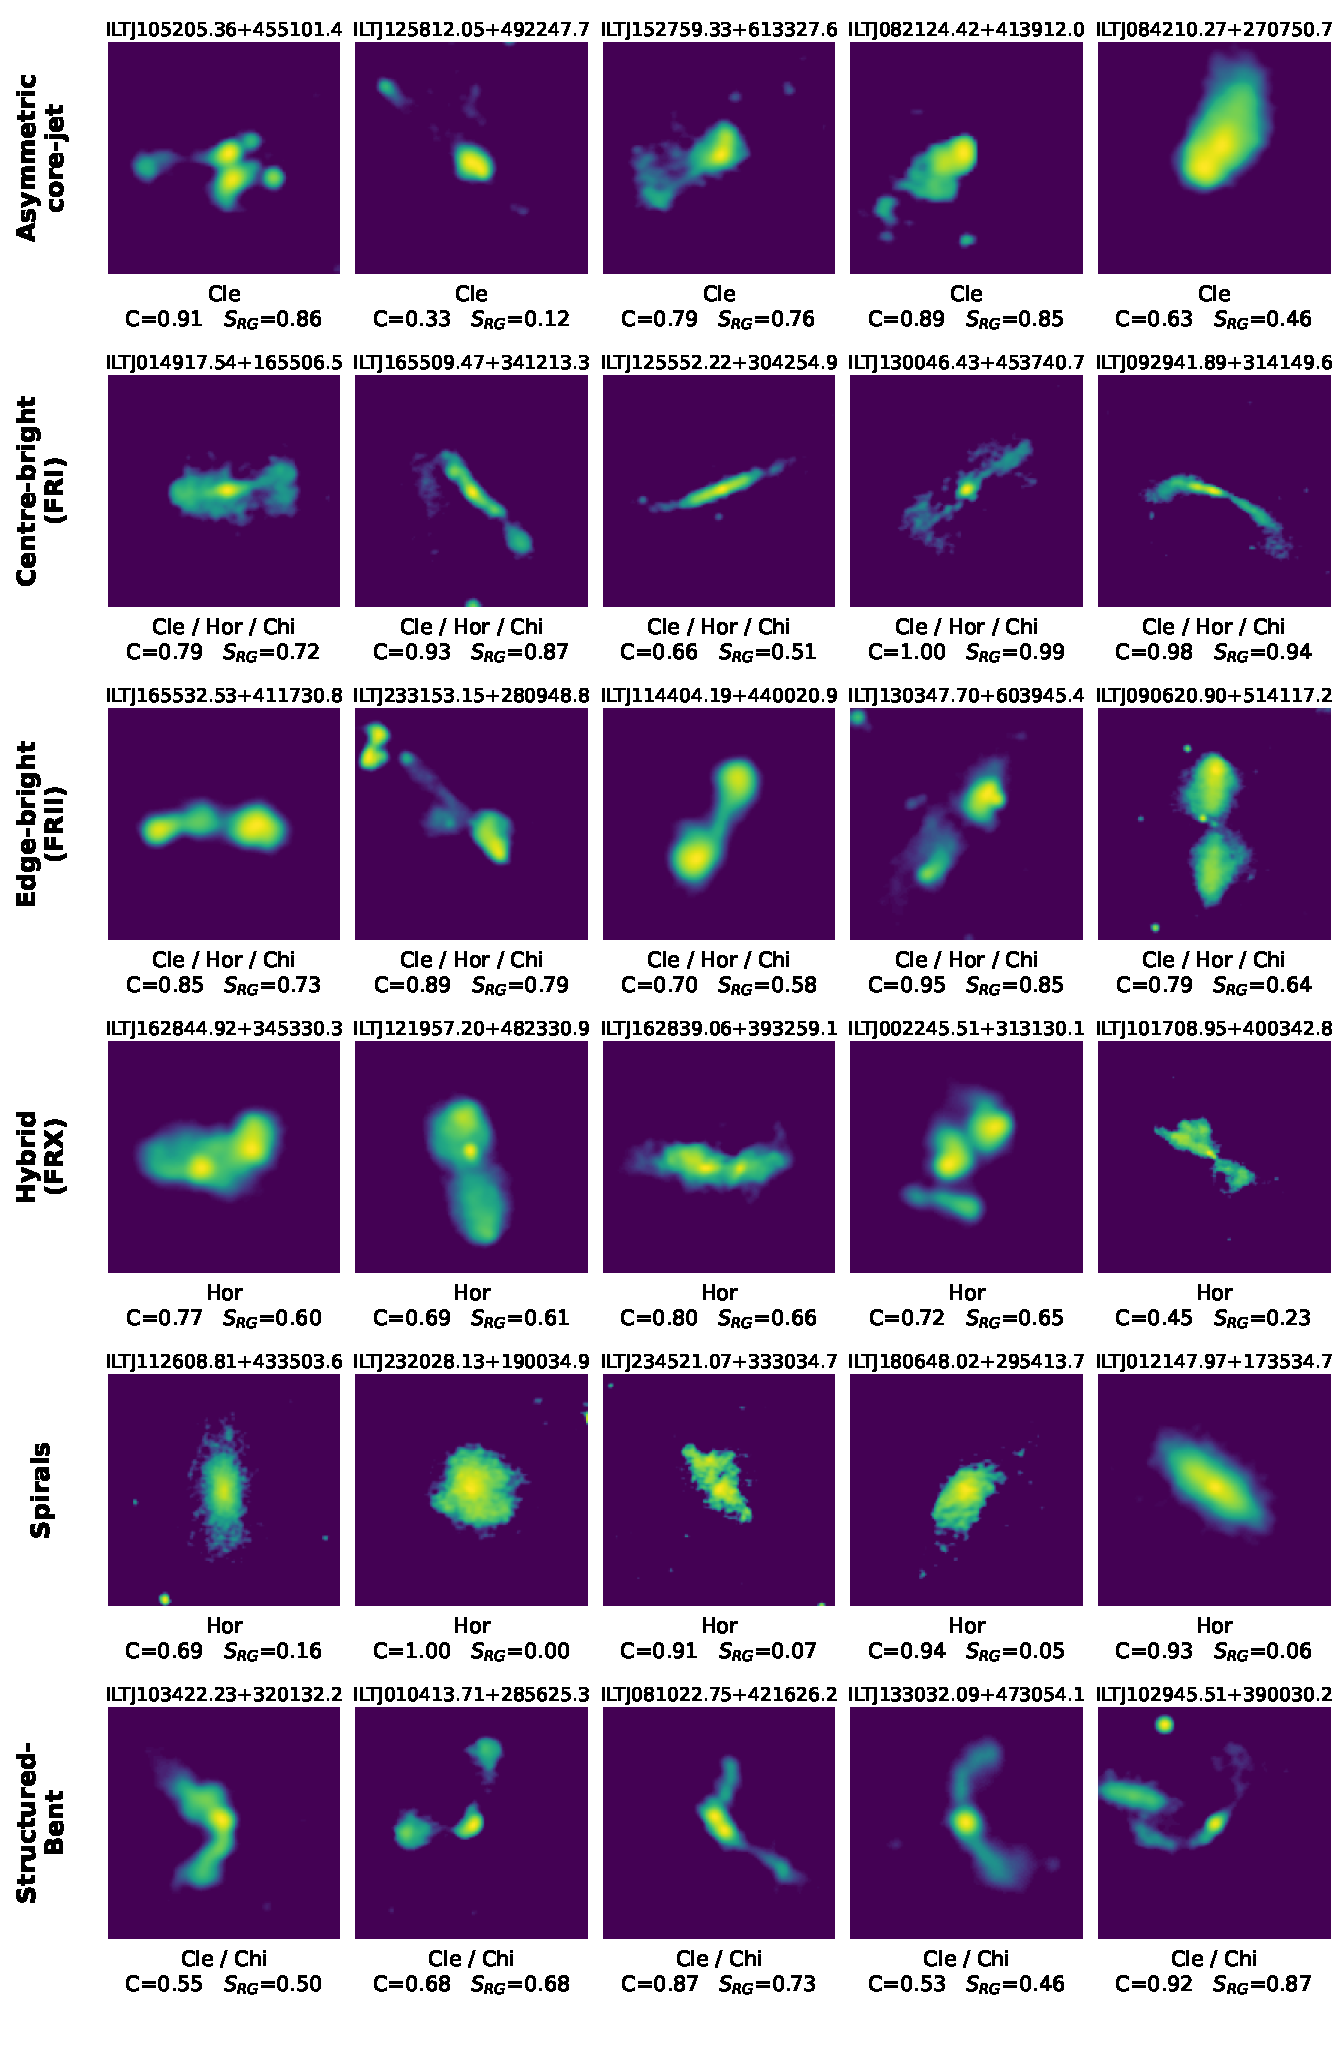
\includegraphics[width=\linewidth,height=0.90\textheight,keepaspectratio]{img/external_agreement_gallery.pdf}
\caption[Examples of agreement with external catalogues]{Agreement examples grouped by ensemble class. Cle, Hor, and Chi identify supporting catalogues. \(C\) denotes confidence and \(S_\mathrm{RG}\) the morphology score.}
\label{fig:agree_gallery}
\end{figure}
